\documentclass[12pt,letterpaper]{article}

\usepackage{amsfonts}
\usepackage{graphics}
\usepackage{graphicx}
\usepackage{colortbl}
\usepackage{amsmath}

\usepackage{algorithm}
\usepackage[noend]{algpseudocode}
\usepackage{array}

\usepackage{epstopdf}

\setlength\intextsep{10pt}
\setlength\textfloatsep{10pt}

\newenvironment{proof}{\noindent{\bf Proof:}}{\qed\bigskip}

\newtheorem{theorem}{Theorem}
\newtheorem{corollary}{Corollary}
\newtheorem{lemma}{Lemma} 
\newtheorem{claim}{Claim}
\newtheorem{fact}{Fact}
\newtheorem{definition}{Definition}
\newtheorem{assumption}{Assumption}
\newtheorem{observation}{Observation}
\newtheorem{example}{Example}
\newcommand{\qed}{\rule{7pt}{7pt}}

\newcommand{\assignment}[4]{
\thispagestyle{plain} 
\newpage
\setcounter{page}{1}
\noindent
\begin{center}
\framebox{ \vbox{ \hbox to 6.28in
{\bf CS578/STAT590: Introduction Machine Learning \hfill #1}
\vspace{4mm}
\hbox to 6.28in
{\hspace{2.5in}\large\mbox{Problem Set #2}}
\vspace{4mm}
\hbox to 6.28in
{{\it Handed Out: #3 \hfill Due: #4}}
}}
\end{center}
}

\newcommand{\solution}[4]{
\thispagestyle{plain} 
\newpage
\setcounter{page}{1}
\noindent
\begin{center}
\framebox{ \vbox{ \hbox to 6.28in
{\bf CS578/STAT590: Introduction to Machine Learning \hfill #4}
\vspace{4mm}
\hbox to 6.28in
{\hspace{2.5in}\large\mbox{Problem Set #3}}
\vspace{4mm}
\hbox to 6.28in
{#1 \hfill {\it Handed In: #2}}
}}
\end{center}
\markright{#1}
}



\def\Comment#1{\textsf{\textsl{$\langle\!\langle$#1\/$\rangle\!\rangle$}}}



\oddsidemargin 0in
\evensidemargin 0in
\textwidth 6.5in
\topmargin -0.5in
\textheight 9.0in

\begin{document}

\solution{Gen Nishida}{\today}{3}{Fall 2014}
% Fill in the above, for example, as follows:
% \solution{John Smith}{\today}{1}{Fall 2014}

\pagestyle{myheadings}  % Leave this command alone

\section{Questions}

\begin{enumerate}
\item Fitting an SVM classifier by hand (source: Machine Learning, a probabilistic perspective. K Murphy)

\begin{enumerate}
\item Write down a vector that is parallel to the optimal vector w.

The decision boundary is perpendicular to the vector $\phi(x_2)-\phi(x_1)$.
\[
\phi(x_2)-\phi(x_1)=[1, 2, 2]^T-[1, 0, 0]^T=[0, 2, 2]^T
\]
Thus, the vector that is parallel to the optimal vector $w$ is $[0, 1, 1]^T$.

\item What is the value of the margin that is achieved by this $w$?

The maximum margin is the half of the distance between two points in the 3d feature space. Thus,
\[
\frac{\|\phi(x_2)-\phi(x_1)\|}{2}=\frac{\|[0, 2, 2]^T\|}{2}=\sqrt{2}
\]

\item Solve for $w$, using the fact the margin is equal to $1/\|w\|$.

Let $w=k [0, 1, 1]^T$. Then,
\[
\|w\|=k\|[0, 1, 1]^T\|=\sqrt{2}k
\]
Since the margin is $\sqrt{2}$,
\[
\sqrt{2}=\frac{1}{\|w\|}=\frac{1}{\sqrt{2}k}
\]
By solving this, we obtain $k=1/2$. Thus, $w=[0, 1/2, 1/2]^T$.

\item Solve for $w_0$ using your value for $w$ and Equations 1 to 3.

By substituting $w$ of Equations 2 and 3, we get
\[
\begin{cases}
y_1(w^T\phi(x_1)+w_0)=-([0, 1/2, 1/2]^T \cdot [1, 0, 0]^T+w_0)=-w_0\ge 1 \\
y_2(w^T\phi(x_2)+w_0)=([0,1/2,1/2]^T \cdot [1, 2, 2]^T+w_0)=2+w_0\ge 1
\end{cases}
\]
By solving this, we obtain
\[
-1\le w_0 \le -1
\]
Thus, $w_0=-1$.

\item Write down the form of the discriminant function $f(x)=w_0+w^T\phi(x)$ as an explicit function of $x$.

\[
f(x)=w_0 + w^T \phi(x)=-1 + [0, 1/2, 1/2]^T \cdot [1, \sqrt{2}x, x^2]^T=\frac{1}{2}x^2+\frac{1}{\sqrt{2}}x-1
\]

\end{enumerate}

\item We define a concept space C that consists of the union of $k$ disjoint intervals in a real line. A concept in C is represented therefore using $2k$ parameters: $a_1 \le b_1 \le a_2 \le b_2 \le \cdots \le a_k \le b_k$. An example (a real number) is classified as positive by such concept iff it lies in one of the intervals. Give the VC dimension of H (and prove its correctness).

The answer is $2k$.

{\bf Proof:}

Let $VC(k)$ be the VC dimension for $k$ disjoint intervals in a real line. I prove by indiction that $VC(k)=2k$ in the following. When $k=1$, two examples have four patterns in total, and all the cases can be correctly classified (Figure \ref{fig:vc_dimension1}). Thus, $VC(1)=2$, which satisifies the above hypothesis. 

\begin{figure}[hbtp]
\centering
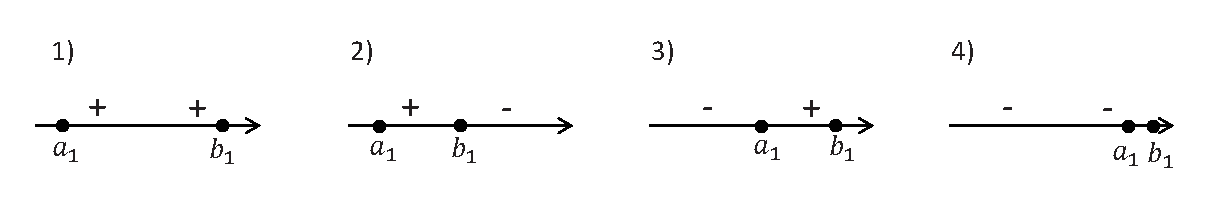
\includegraphics[width=150mm]{vc_dimension1}
\caption{For the case of $k=1$, two examples are correctly classified in all the four cases. Thus, $VC(1)=2$.}
\label{fig:vc_dimension1}
\end{figure}

Now, given that $VC(k-1)=2(k-1)$, we want to show that two additional examples can be correctly classified by an additional interval. Assume without loss of generality that two additional numbers are greater than the existing $2(k-1)$ ones that are already classified. Then, there are only four cases in terms of the labels of two additional examples, and they are correctly classified by $k$-th interval in all cases (Figure \ref{fig:vc_dimension2}). 
\begin{figure}[hbtp]
\centering
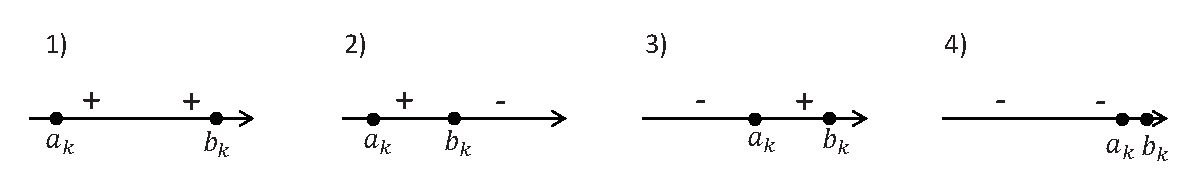
\includegraphics[width=150mm]{vc_dimension2}
\caption{When adding $k$-th interval, two additional examples are correctly classified in all the four cases.}
\label{fig:vc_dimension2}
\end{figure}

Thus, 
\[
VC(k) \ge VC(k-1)+2=2(k-1)+2=2k
\]
Therefore, $VC(k)$ is at least $2k$ by induction. Also, Figure \ref{fig:vc_dimension3} shows a case in which $k+1$ positive examples and $k$ negative examples cannot be correctly classified. This concludes $VC(k) = 2k$.
\begin{figure}[hbtp]
\centering
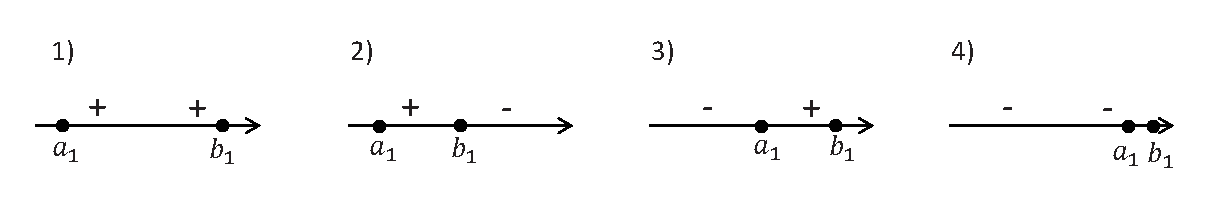
\includegraphics[width=140mm]{vc_dimension3}
\caption{This figure shows a case in which $k+1$ positive examples and $k$ negative examples cannot be correctly classified by $k$ disjoint intervals. The right most positive example (red color) is classified incorrectly. Thus, $VC(k) < 2k+1$.}
\label{fig:vc_dimension3}
\end{figure}


\item The Gradient Descent (GD) algorithm

\begin{enumerate}
\item Write in one sentence: what are the hyper parameters of the GD algorithm.

The hyper parameters are the initial weight vector which you can randomly initialize if you want, learning rate that is the step size of updating the weight vector, a parameter $\lambda$ that defines the impact of the regularizer, and the convergence criteria when to stop the iteration such as the maximum number of iterations.

\item Write in one sentence: What is the difference between $l1$ and $l2$ regularization.

$l1$ regularization uses $l1$ norm of $w$ as the regularization term, which encourages the sparsity, while $l2$ regularization uses $l2$ norm of $w$.

\item Write down the gradient descent algorithm applied to hinge loss with $l2$ regularization.

The objective function is
\[
F(w)=\frac{\lambda}{2}\|w\|^2+\sum_i \max{(0, 1-y_i (w^Tx_i+b))}
\]
Then, its partial derivative with regard to $w$ and $b$ are
\[
\frac{\partial F(w)}{w}=\lambda w+ \sum_i
\begin{cases}
-y_i x_i & ({\rm if} \; y_i(w^Tx_i+b) \le 1) \\
0 & {\rm Otherwise}
\end{cases}
\]
and
\[
\frac{\partial F(w)}{b}=\sum_i
\begin{cases}
-y_i & ({\rm if} \; y_i(w^Tx_i+b) \le 1) \\
0 & {\rm Otherwise}
\end{cases}
\]

\begin{algorithm}
\caption{Gradient descent algorithm applied to hige loss with l2 regularization}\label{euclid}
\begin{algorithmic}[1]
\Procedure{HingeRegularizedGD()}{}
\State Initialize $w$ and $b$ randomly
\For{$i=0$ to $maxIterations$}
\State $\Delta w=(0, \cdots, 0)$
\State $\Delta b=0$
\ForAll{training data $x_d$ for $d = 1,\cdots,D$}
\If{$y_d w \cdot x_d + b \le 1$}
\State $\Delta w= \Delta w+y_d x_d$
\State $\Delta b=\Delta b+y_d$
\EndIf
\EndFor
\State $\Delta w=\Delta w - \lambda w$
\State $w=w+\eta \Delta w$
\State $b=b+\eta \Delta b$
\State \Return $w$ and $b$ when they have converged
\EndFor
\EndProcedure
\end{algorithmic}
\end{algorithm}

The algorithm is shown in Algorithm 1. Note that the bias term is included in the weight vector by extending the feature vector as $[x, 1]^T$ and the weight vector as $[w, b]^T$.



\end{enumerate}

\end{enumerate}

\section{Programming Assignment}

For the programming assignment, I used SVM with the hinge loss function and $l1$ or $l2$ regularization as required. The pseudo code of gradient descent algorithm to solve this is shown in Algorithm 2, which is basically similar to Algorithm 1 except that both $l1$ and $l2$ are supported.

\begin{algorithm}
\caption{Gradient descent algorithm applied to hige loss with l1 and l2 regularization}\label{euclid}
\begin{algorithmic}[1]
\Procedure{GD(maxIterations, regularization, $\eta$, $\lambda$)}{}
\State Initialize $w$ and $b$ randomly
\For{$iter=0$ to $maxIterations$}
\State $\Delta w=(0, \cdots, 0)$
\State $\Delta b=0$
\ForAll{training data $x_d$ for $d = 1,\cdots,D$}
\If{$y_d w \cdot x_d + b \le 1$}
\State $\Delta w= \Delta w+y_d x_d$
\State $\Delta b=\Delta b+y_d$
\EndIf
\EndFor
\If{regularization == $l1$}
\For{$i=0$ to $N$}
\If{$w_i \ge 0$}
\State $\Delta w_i=\Delta w_i-\lambda$
\Else
\State $\Delta w_i=\Delta w_i+\lambda$
\EndIf
\EndFor
\ElsIf{regularization == $l2$}
\State $\Delta w=\Delta w - \lambda w$
\EndIf
\State $w=w+\eta \Delta w$
\State $b=b+\eta \Delta b$
\State \Return $w$ and $b$ when they have converged
\EndFor
\EndProcedure
\end{algorithmic}
\end{algorithm}

\subsection*{Feature Set}
For the continuous values, I used all the intervals between two consequtive thresholds as attributes. For instance, if an original attribute $a$ has three thresholds ${1, 2, 3}$, then the corresponding attributes will be $\{(a<1),(a\ge 1; a<2),(a\ge 2; a<3),(a\ge 3)\}$. Also, I ignored the examples that contain missing values.

\subsection*{Hyper Parameters}
There are five hyper parameters, $maxIterations$, $l1$ or $l2$, $stepSize$, $lambda$, and feature set. Unlike Perceptron algorithm, my objective function includes regularization term that somewhat avoids the overfitting. Thus, I used a very large number for maxIterations, say 20000 to get the gradient descent converged without worrying about the overfiting. For each combination of $regularization$ and $featureSet$, I used a set $\{0.0001, 0.001, 0.01, 0.1, 1\}$ for $stepSize$ and a set $\{0.0001, 0.001, 0.01, 0.1, 1\}$ for $lambda$ to find the best combination. The results are shown in Figure ?. Based on the results, I chose the combination of $stepSize$ and $labmda$ as shown in Figure ?.

\subsection*{Results}
Using the selected hyperparameters, I experimented the learned hypothesis over the test data.

\begin{figure}[hbtp]
\centering
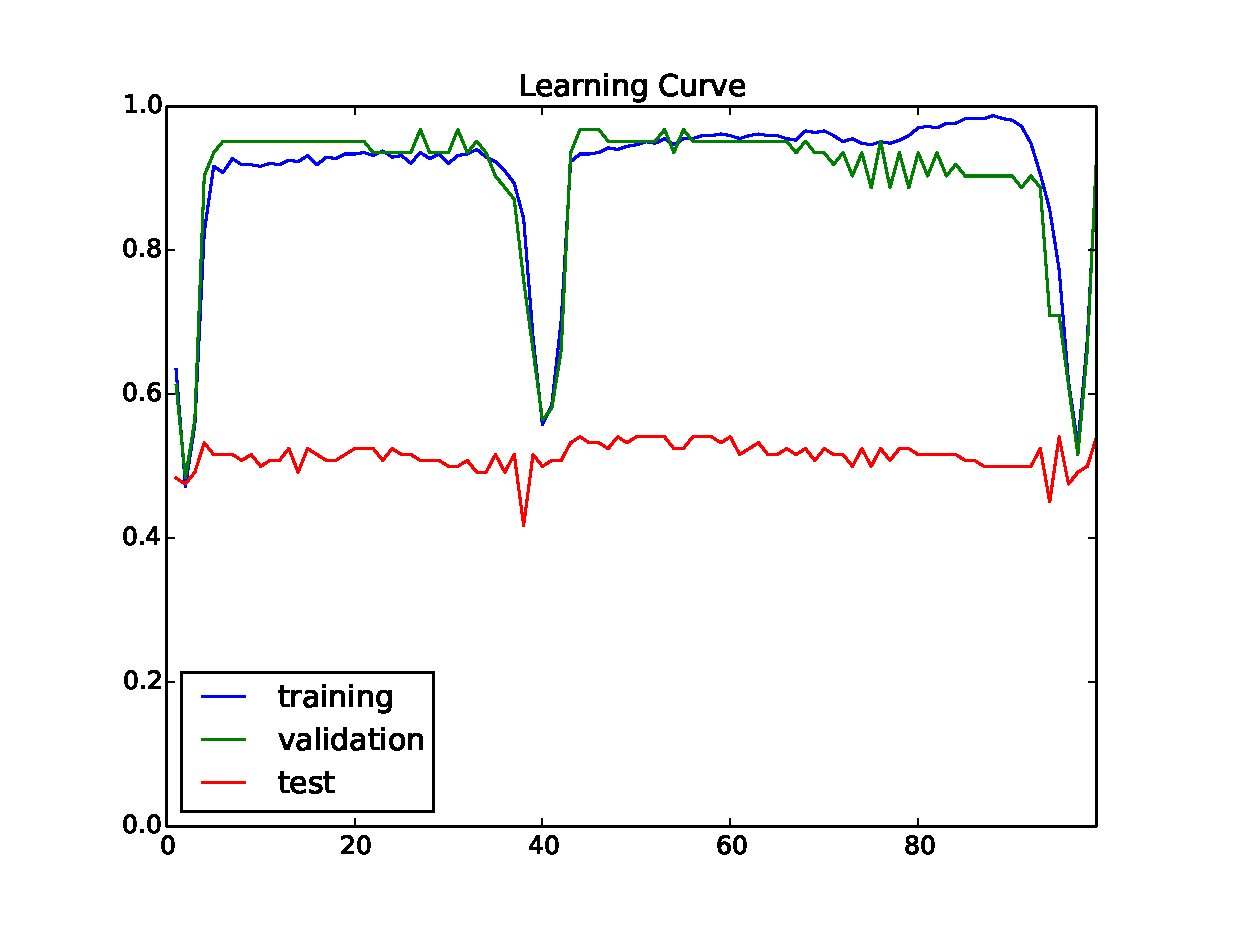
\includegraphics[width=140mm]{learning_curve_l1_1}
\caption{This figure shows the learning curve with $l1$ regularization and $featureSet=1$.}
\label{fig:learning_curve_l1_1}
\end{figure}

\begin{figure}[hbtp]
\centering
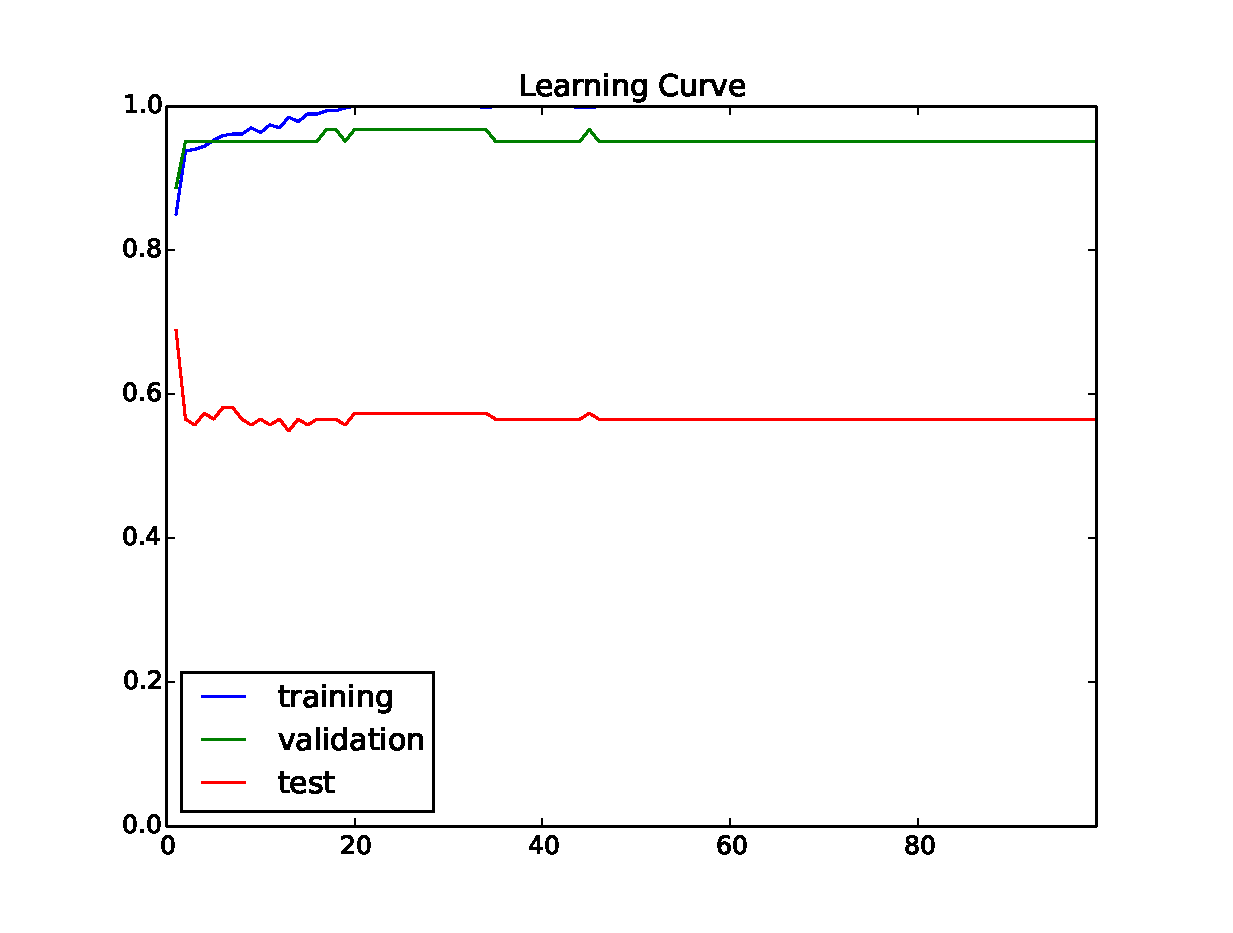
\includegraphics[width=140mm]{learning_curve_l2_1}
\caption{This figure shows the learning curve with $l2$ regularization and $featureSet=1$.}
\label{fig:learning_curve_l2_1}
\end{figure}

\end{document}

